% Created 2016-10-23 Sun 18:35
% Intended LaTeX compiler: pdflatex
\documentclass[a4paper, twoside]{article}
\usepackage[utf8]{inputenc}
\usepackage[T1]{fontenc}
\usepackage{graphicx}
\usepackage{grffile}
\usepackage{longtable}
\usepackage{wrapfig}
\usepackage{rotating}
\usepackage[normalem]{ulem}
\usepackage{amsmath}
\usepackage{textcomp}
\usepackage{amssymb}
\usepackage{capt-of}
\usepackage{hyperref}
\usepackage{pdflscape}
\usepackage{booktabs}
\usepackage{lscape, subfigure, graphicx}
\usepackage{minted}
\usemintedstyle{autumn}
\newminted{sh}{fontsize=\footnotesize}
\usepackage{hyperref}
\hypersetup{
colorlinks,%
citecolor=black,%
filecolor=black,%
linkcolor=black,%
urlcolor=blue}%
\let\tmp\oddsidemargin
\let\oddsidemargin\evensidemargin
\let\evensidemargin\tmp
\reversemarginpar
\makeatletter
\renewcommand{\l@section}{\@dottedtocline{1}{2em}{2em}}
\renewcommand{\l@subsection}{\@dottedtocline{2}{4em}{4em}}
\renewcommand{\l@subsubsection}{\@dottedtocline{3}{6em}{5em}}
\makeatother
\author{senthil}
\date{\today}
\title{Using org-mode in research}
\hypersetup{
 pdfauthor={senthil},
 pdftitle={Using org-mode in research},
 pdfkeywords={},
 pdfsubject={},
 pdfcreator={Emacs 25.1.1 (Org mode 8.3.4)}, 
 pdflang={English}}
\begin{document}

\maketitle

\section{Introduction}
\label{sec:org5a75567}
\begin{itemize}
\item Emacs is a text editor (short for Editor MAcroS)
\item Text editors are much more useful than to just display/edit text
\item Plain (UTF-8) text is the best form to preserve data (not a Excel
file not a JPEG image of a plot!)
\item Emacs includes a `mode' called org-mode that is very useful to
organize data and experiments, carry out analysis using scripts
and other external programs and store results and all the
procedures applied to the data in a single location as a simple
text file.
\item Documenting in org-mode is useful in reproducible research.
\end{itemize}
\section{Org-mode in note taking}
\label{sec:org8d57b61}
\subsection{Sections and subsections}
\label{sec:org359347d}
\begin{itemize}
\item Section titles have one `*', two `**' indicate subsection titles
\item Easy to increase or decrease levels of different sectioning
\item 

\item an item in a list (see below)
\item 
\end{itemize}
\subsection{Lists}
\label{sec:org339f4ca}
\subsubsection{Bullet points}
\label{sec:orgd75efda}
\begin{itemize}
\item We already saw how itemized lists are shown in the \ref{sec:org5a75567}
\end{itemize}
\subsubsection{Numbered lists}
\label{sec:orgcd7951e}
\begin{itemize}
\item Numbered lists appear like this:
\begin{enumerate}
\item First item
\item Second item
\item \ldots{}etc.
\item 

\item 

\item 

\item 

\item 
\end{enumerate}
\end{itemize}
\subsubsection{Check list [3/3]}
\label{sec:org24db8e2}
\begin{itemize}
\item $\boxtimes$ Finish first item
\item $\boxtimes$ Then second item
\item $\boxtimes$ Finally do the third item in the check list
\end{itemize}
\subsection{Todo lists [100\%]}
\label{sec:org7d0e6ef}
\subsubsection{{\bfseries\sffamily DONE} Download 16S rRNA sequences from NCBI}
\label{sec:orgb3ea7c0}
\subsubsection{{\bfseries\sffamily DONE} Align to SILVA database using mothur}
\label{sec:org4a3e16d}
\subsubsection{{\bfseries\sffamily DONE} Manually curate using BioEdit, SeaView, etc.}
\label{sec:org51a675}
\subsubsection{{\bfseries\sffamily DONE} Apply hard and soft filter}
\label{sec:orge33981f}
\subsubsection{{\bfseries\sffamily DONE} Calculate distance matrix, construct NJ tree}
\label{sec:orgfdd849a}
\subsubsection{{\bfseries\sffamily DONE} Construct ML and MP tree}
\label{sec:org6d893d0}
\subsubsection{{\bfseries\sffamily DONE} Edit trees in iTOL}
\label{sec:orgc11b234}
\subsubsection{{\bfseries\sffamily DONE} Beautify in Inkscape or Illustrator}
\label{sec:orgdcaa0fb}

\subsection{Tables}
\label{sec:org7a119bd}
\begin{itemize}
\item Tables can be created by hand
\item Spreadsheet like capablities
\end{itemize}

\begin{center}
\begin{tabular}{lr}
\hline
Subject & Score\\
\hline
Phy & 90\\
Chem & 89\\
Biol & 70\\
Math & 79\\
\hline
Total & 249\\
\hline
Avg & 83\\
\hline
\end{tabular}
\end{center}

\begin{itemize}
\item Tables can also be created from tab-limited or csv-limited text
\item Use command: \texttt{M-x org-table-convert-region}
\end{itemize}

\begin{center}
\begin{tabular}{lrrrrrrr}
\hline
bin & N50 & size & ctgs & genes & markers & \%cov & dup\_mark\\
\hline
b1\_m4 & 6467 & 7.29 & 1708 & 8588 & 136 & 108 & 294\\
b2\_m4 & 5206 & 5.96 & 1609 & 6954 & 38 & 30 & 23\\
hi\_m4 & 21756 & 1.78 & 123 & 1979 & 58 & 46 & 5\\
meta\_m4 & 4738 & 61.25 & 20730 & 76130 & 139 & 111 & 1407\\
\hline
\end{tabular}
\end{center}

\subsection{Figures}
\label{sec:orgcc84880}
\section{Org-mode in reproducible research}
\label{sec:org1202360}
\subsection{Many published results not reproducible}
\label{sec:org8cee4a}
\begin{itemize}
\item A figure or a plot is useful to describe results
\item 53 deliberately chosen cancer research papers (novel approaches)
\item Only 6 were reproducible (11 \% cases)
\item 73 \% authors: NO RESPONSE to data request (Psychology)
\end{itemize}
\subsection{Solution: Include data with your figures}
\label{sec:org4fd6e54}
\begin{itemize}
\item The following illustrate a trivial example
\item But there are real world examples (see email)
\end{itemize}
\subsection{Toy example}
\label{sec:orgac521a}
\begin{itemize}
\item 454 reads assembled using genome assembly program (Newbler)
\item Two varying parameters:
\begin{itemize}
\item Minimum overlap length in bp(ml): 5, 10, 20, 30, 40, 50
\item Minimum percentage identity (mi): 75, 80, 85, 90, 95
\end{itemize}
\item The following snippets of code runs newbler gets the stats
\end{itemize}
\subsubsection{Newbler assembly}
\label{sec:org78fef15}
\begin{minted}[]{sh}
# /mnt/hit2g/senthil_files/PYROPHAGE/bin/try_runassembly.sh
#!/bin/bash
# Senthil / UNLV / October 14, 2014
# Try different -ml and -mi values for assembling pyrophage data
for mi in 75 80 85 90 95;
do
    for ml in 5 10 20 30 40 50;
    do
	# with urt
	runAssembly -o ../results/URT_NEW_PYRO_${mi}_${ml} -force \
	    -ml ${ml} -mi ${mi} -nobig -cpu 6 -urt \
	    ../data/Hot_Springs_metagenome_G7162.fasta;
    done
done
\end{minted}
\subsubsection{Get assembly stats}
\label{sec:orge79e765}
\begin{itemize}
\item Use R to check assembly statistics
\item Extract stats to output file
\end{itemize}
\begin{minted}[]{sh}
for i in $(find ../results/ -name "454AllContigs.fna");
do 
    j=$(echo $i | cut -d "/" -f 3);
    k1=$(echo ${j} | cut -d"_" -f 4);
    k2=$(echo ${j} | cut -d "_" -f 5);
    k3=$(echo $j | cut -d "_" -f 1);
    echo -ne "${j}\t${k1}\t${k2}\t\"${k3}\"\t";
    read_fasta -i ${i} | analyze_assembly -x \
	| cut -d ":" -f 2 | tr '\n' '\t' | sed -e 's/---//g';
    echo;
done > urt.out;
\end{minted}
\subsubsection{Experimental output table}
\label{sec:org908453b}
\begin{center}
\label{tab:org873c812}
\begin{tabular}{lrrrrrr}
\hline
name & mi & ml & n50 & lc & asize & ctgs\\
\hline
URT\_NEW\_PYRO\_95\_20 & 95 & 20 & 1686 & 17476 & 8327669 & 7880\\
URT\_NEW\_PYRO\_95\_30 & 95 & 30 & 1628 & 17514 & 8246873 & 8012\\
URT\_NEW\_PYRO\_80\_30 & 80 & 30 & 1571 & 15253 & 8427227 & 8594\\
URT\_NEW\_PYRO\_95\_5 & 95 & 5 & 1733 & 17514 & 8294156 & 7524\\
URT\_NEW\_PYRO\_95\_50 & 95 & 50 & 1511 & 17486 & 8058979 & 8446\\
URT\_NEW\_PYRO\_75\_50 & 75 & 50 & 1471 & 16189 & 8256061 & 8971\\
URT\_NEW\_PYRO\_75\_5 & 75 & 5 & 1677 & 17515 & 8490416 & 8100\\
URT\_NEW\_PYRO\_95\_10 & 95 & 10 & 1733 & 17476 & 8290778 & 7563\\
URT\_NEW\_PYRO\_75\_40 & 75 & 40 & 1526 & 15253 & 8340378 & 8746\\
URT\_NEW\_PYRO\_80\_10 & 80 & 10 & 1679 & 17515 & 8499064 & 8069\\
URT\_NEW\_PYRO\_85\_40 & 85 & 40 & 1528 & 15253 & 8314699 & 8702\\
URT\_NEW\_PYRO\_80\_40 & 80 & 40 & 1528 & 11866 & 8333476 & 8752\\
URT\_NEW\_PYRO\_85\_20 & 85 & 20 & 1624 & 15253 & 8535743 & 8465\\
URT\_NEW\_PYRO\_80\_50 & 80 & 50 & 1472 & 15253 & 8246656 & 8947\\
URT\_NEW\_PYRO\_90\_10 & 90 & 10 & 1681 & 17515 & 8494919 & 8079\\
URT\_NEW\_PYRO\_85\_50 & 85 & 50 & 1472 & 15253 & 8245814 & 8930\\
URT\_NEW\_PYRO\_75\_20 & 75 & 20 & 1623 & 15253 & 8533799 & 8483\\
URT\_NEW\_PYRO\_85\_30 & 85 & 30 & 1569 & 15253 & 8432496 & 8618\\
URT\_NEW\_PYRO\_85\_10 & 85 & 10 & 1677 & 17553 & 8499299 & 8089\\
URT\_NEW\_PYRO\_90\_20 & 90 & 20 & 1619 & 15253 & 8528845 & 8487\\
URT\_NEW\_PYRO\_85\_5 & 85 & 5 & 1677 & 17515 & 8492951 & 8077\\
URT\_NEW\_PYRO\_90\_30 & 90 & 30 & 1577 & 15253 & 8423223 & 8583\\
URT\_NEW\_PYRO\_95\_40 & 95 & 40 & 1575 & 17486 & 8125789 & 8085\\
URT\_NEW\_PYRO\_75\_30 & 75 & 30 & 1578 & 14477 & 8420677 & 8547\\
URT\_NEW\_PYRO\_90\_50 & 90 & 50 & 1477 & 15253 & 8231116 & 8889\\
URT\_NEW\_PYRO\_80\_5 & 80 & 5 & 1677 & 13349 & 8496575 & 8092\\
URT\_NEW\_PYRO\_75\_10 & 75 & 10 & 1677 & 17553 & 8498313 & 8074\\
URT\_NEW\_PYRO\_80\_20 & 80 & 20 & 1617 & 16530 & 8547131 & 8506\\
URT\_NEW\_PYRO\_90\_5 & 90 & 5 & 1680 & 17515 & 8490953 & 8065\\
URT\_NEW\_PYRO\_90\_40 & 90 & 40 & 1528 & 15253 & 8330050 & 8703\\
\hline
\end{tabular}
\end{center}
\subsubsection{Plot}
\label{sec:orgc3bed55}
\begin{minted}[]{r}
library(ggplot2)
mydat <- read.table('urt.out', head=T, row.names=1)
pdf('n50_ovlgth.pdf', useDingbats=FALSE)
p <- ggplot(mydat, aes(ml, n50)) +
    geom_point(aes(colour=factor(mi))) +
    xlab('Seq overlap (bp)') +
    ylab('N50 (bp)')
p <- p + labs(colour='% identity')
p + ggtitle('Sequence identity and overlap vs N50')
dev.off()
\end{minted}
\subsection{Final result}
\label{sec:org596e795}
\begin{figure}[htb]
\centering
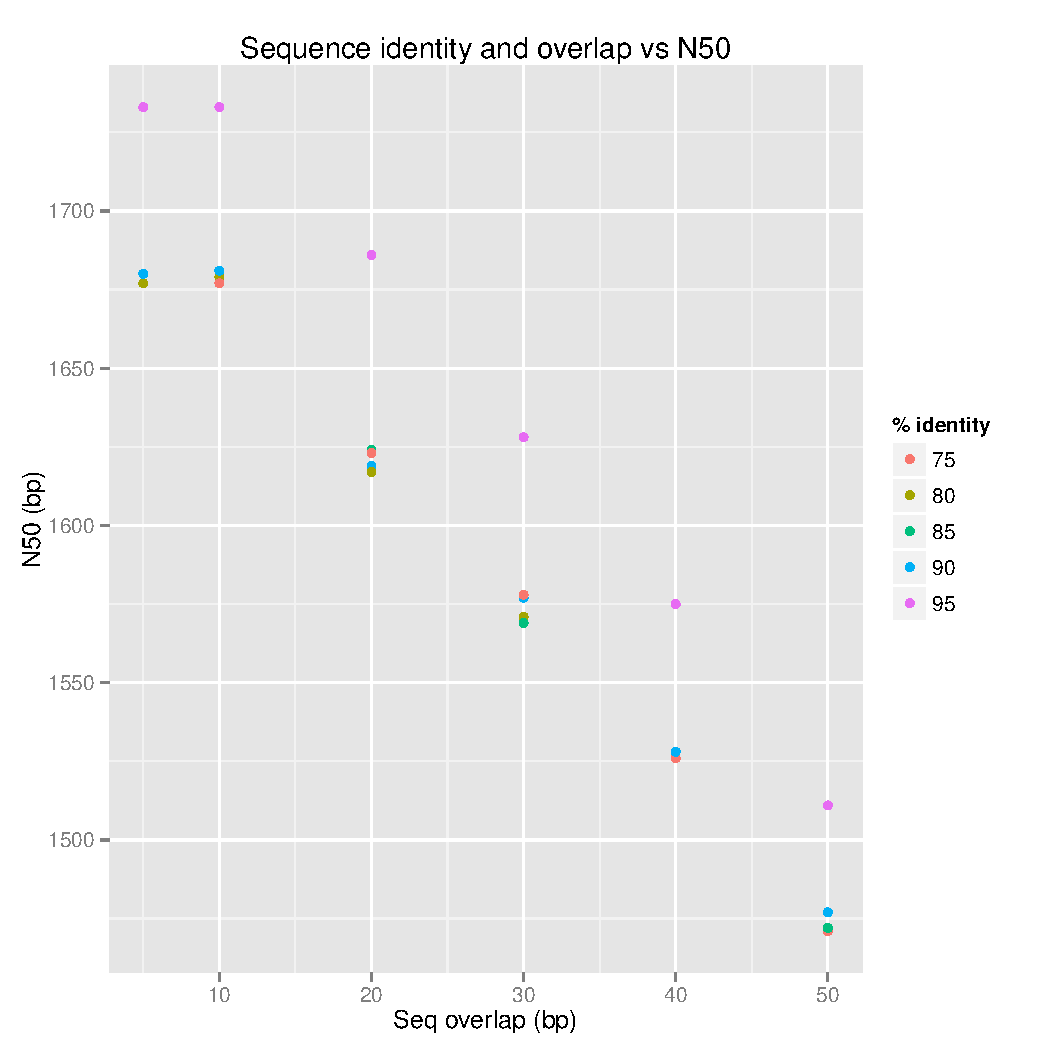
\includegraphics[width=.9\linewidth]{./n50_ovlgth.pdf}
\caption{\label{fig:org7b0ff08}
N50 is inversely related to sequence identity and overlap}
\end{figure}

\begin{itemize}
\item The length of the sequence overlap between reads and the N50 are
inversely related (Fig \ref{fig:org7b0ff08}), higher identity (95\%) resulted in
slightly better N50.
\end{itemize}

\section{Exporting to other formats}
\label{sec:org588133e}
\begin{itemize}
\item So far, we saw how everything is text (scripts, results,
documentation, etc)
\item Org-mode allows exporting the text to PDF, HTML
\item Use \textasciitilde{}C-e C-l C-p' to get PDF
\item Use \textasciitilde{}C-e C-h C-h' to get HTML
\end{itemize}
\end{document}
